\documentclass[utf8,a4paper,12pt]{article}
\usepackage[utf8]{inputenc}
\usepackage[russian]{babel}
\usepackage[]{amsmath,amssymb,textcomp,amsthm}
\usepackage{float}
\usepackage{tikz}
\usepackage[inline]{enumitem}
\usepackage[final]{pdfpages}
%\usepackage{mathptmx}
\newtheorem{lemma_cub}{Лемма}[section]
\title{Группа, порожденная поворотами двух смежных граней кубика Рубика}
\author{}
\date{}
\begin{document}
%% Title page
%%
\begin{center}
{\scshape Специализированный учебно-научный центр (факультет) – школа-интернат имени А.Н.Колмогорова Московского государственного университета имени М.В.Ломоносова\par}
\par\vfill
\vspace{1.5cm}
{\Large\bfseries
Группа, порожденная поворотами двух смежных граней кубика Рубика
\par}
\vspace{1.5cm}
\par\vfill
\noindent\hspace{0.52\textwidth}\parbox[t]{0.48\textwidth}{
Исследовательская работа\\[3pt]
ученика 11 ''Л'' класса\\[3pt]
Нечаева Егора Тимофеевича\\[3pt]
03.05.2001\\[3pt]
+7 (999) 868-68-13\\[3pt]
nechaev.e.01@gmail.com\\[3pt]
СУНЦ МГУ, Москва.\\[3pt]
Научный руководитель:\\[3pt]
кандидат физико-математических наук, доцент СУНЦ МГУ\\
Дубровский Владимир Натанович.\\[2ex]
}
\par\vfill
Москва 2019
\end{center}
\thispagestyle{empty}
\pagebreak
%%
%% ===========================================================================
%%
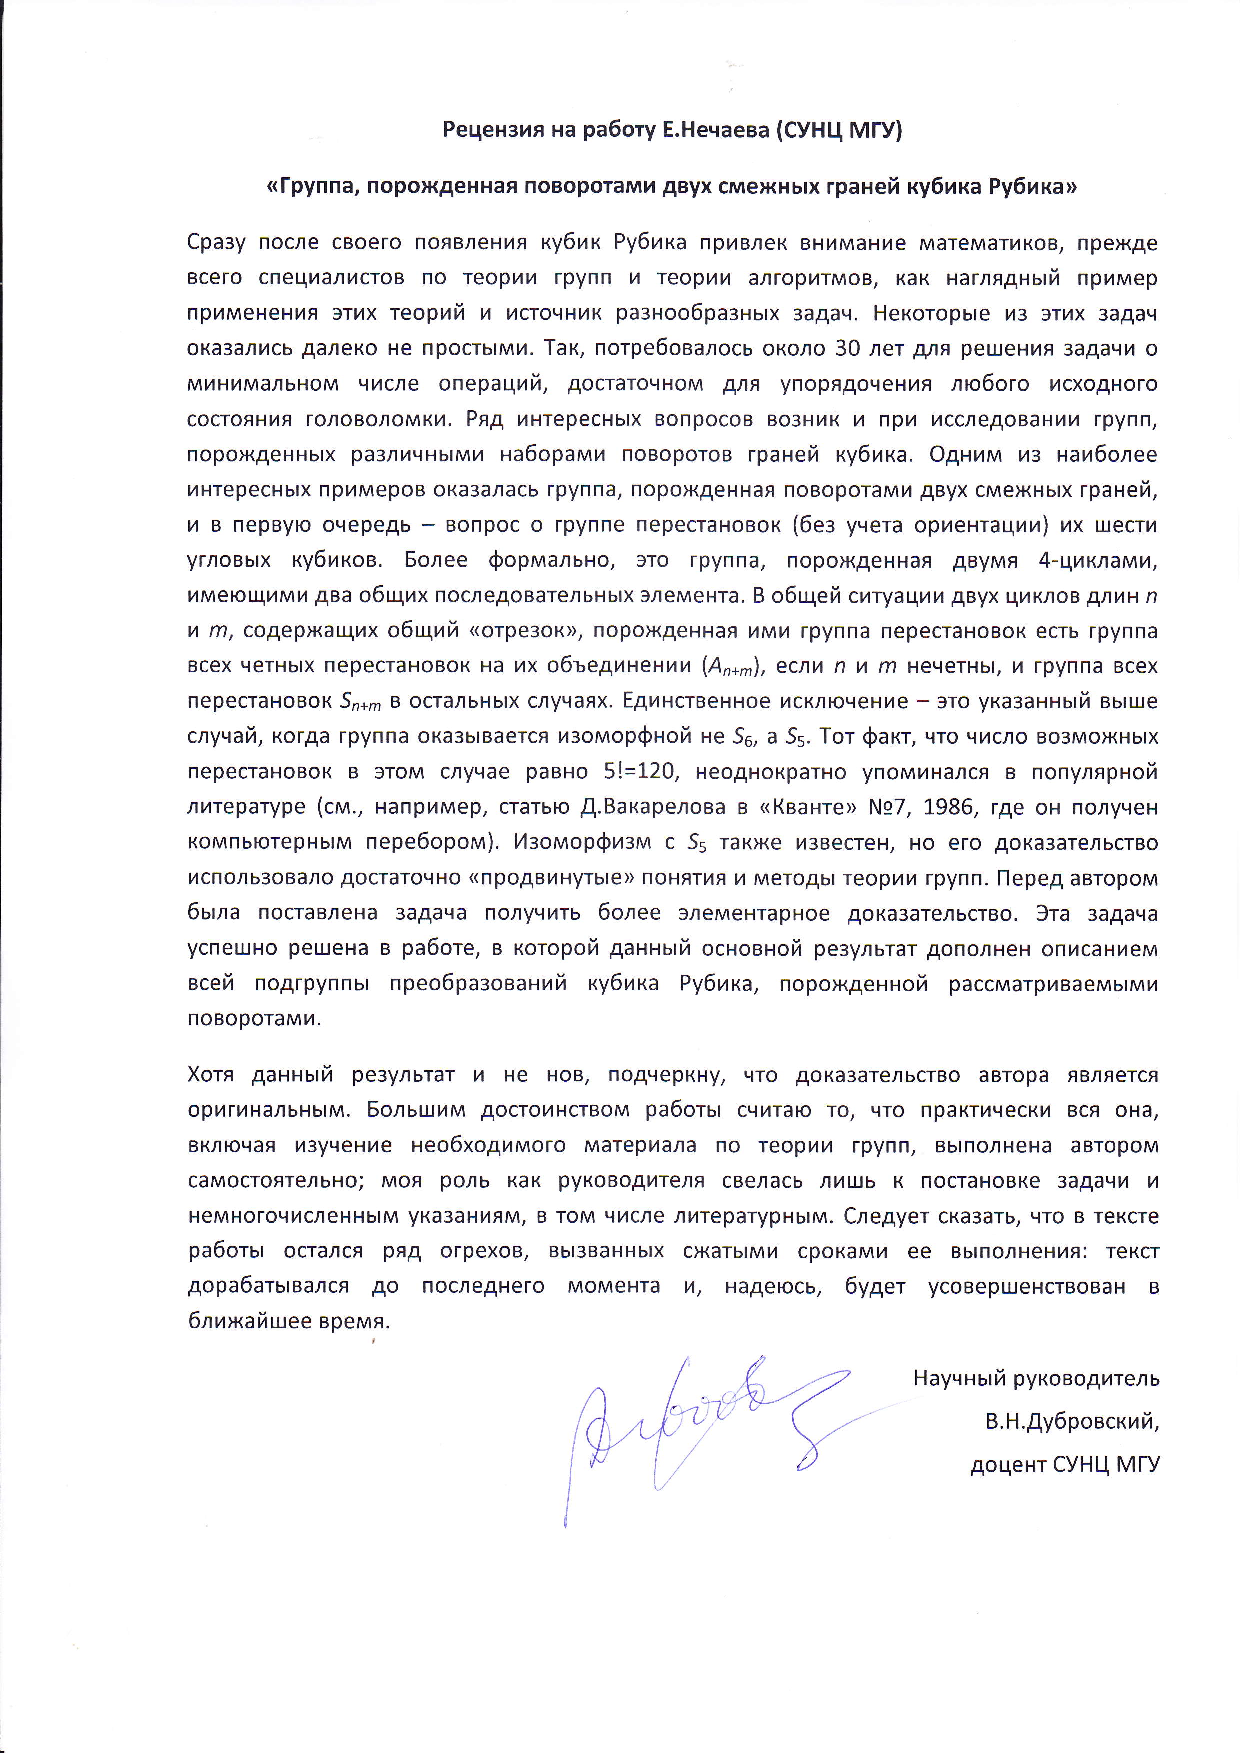
\includepdf[pages=-]{reviewpdf.pdf}
\begin{abstract}
В работе исследована группа, порожденная поворотами двух смежных граней кубика Рубика с помощью исследования связанных с ней групп движения отдельных элементов двух граней~--- угловых и реберных кубиков. Доказано, что группа перестановок реберных кубиков изоморфна $S_7$, группа поворотов тривиальна, группа перестановок угловых кубиков изоморфна $S_5$, группа поворотов изоморфна $\mathbb{Z}_3^5$. Получено полное описание группы: $\mathbb{Z}_3^5\times ((A_5\times A_7)\rtimes\mathbb{Z}_2)$.
\end{abstract}
\section{Введение}
Цель данной работы~--- исследовать одну из подгрупп группы кубика Рубика, порожденную поворотами только двух смежных граней. Особенно интересна тесно связанная с ней группа перестановок шести угловых кубиков этих граней, порожденная теми же поворотами: естественное предположение о том, что эта группа совпадает с группой $S_6$ всех перестановок углов оказывается неверным.

Задачей этой работы будет описание этой группы через прямые и полупрямые произведения симметрических или знакопеременных, и циклических групп. Для исследованая выделим в группе 4 связанные с движением отдельных элементов этих двух граней: группу поворотов реберных кубиков, группу перестановок реберных кубиков, группу поворотов угловых кубиков и группу перестановок угловых кубиков и исследуем каждую из них по отдельности.

У кубика выберем две смежные грани, например, ''верхнюю'' и ''левую'' и обозначим их повороты на 90\textdegree~по часовой стрелке как $U$ и $L$.
\section{Перестановки и повороты реберных кубиков}
Без учета поворотов угловых кубиков, перестановка $U$ поворачивает по кругу реберные кубики $(1,2,3,4)$, перестановка $L$ поворачивает по кругу кубики $(1,5,6,7)$. Тогда перестановка $UL=(1,2,3,4,5,6,7)$ и перестановка $L^{-1}U^2LU^{-1}L^{-1}U^{-1}LU^{-1}=(1,2)$~--- через эти элементы могут быть выражены 2-циклы ($(1~2~\ldots~n)^{-i}(1~2)(1~2~\ldots~n)^i=(i+1~i+2)$)~--- порождающие элементы группы $S_7$~\cite{alexeev}.

Невозможно повернуть центральные кубики. Действительно, выберем ориентацию произвольного реберного кубика и на каждом ребре запишем ориентацию этого кубика, если он двигая его перестановками $U$ и $L$ (рис.~\ref{center_orientations}). Видно, что чтобы поменять ориентацию, нужно выполнить движение третьей стороной (верхней или нижней), а при движениях любой из граней $U$ или $L$ ориентация будет сохраняться. Это значит, что группа поворотов центральных кубиков тривиальна.
\begin{figure}[ht]
\centering
\begin{picture}(50,60)
\put(0,0){\vector(1,0){17}} \put(15,0){\line(1,0){15}}
\put(0,30){\vector(0,-1){17}} \put(0,15){\line(0,-1){15}}
\put(30,30){\vector(-1,0){17}} \put(15,30){\line(-1,0){15}}
\put(30,0){\vector(0,1){17}} \put(30,15){\line(0,1){15}}
\put(0,30){\line(3,2){20}}
\put(50,13){\vector(-3,-2){12}} \put(40,7){\line(-3,-2){10}}
\put(30,30){\vector(3,2){12}} \put(30,30){\line(3,2){20}}
\put(50,43){\vector(0,-1){20}} \put(50,28){\line(0,-1){15}}
\put(19,43){\line(1,0){30}}
\end{picture}
\caption{Ориентации реберного кубика\label{center_orientations}}
\end{figure}
\section{Повороты угловых кубиков}
\begin{lemma_cub}
\label{l_rot}
У любой перестановки можно поменять углы поворотов двух смежных кубиков.
\end{lemma_cub}
\begin{proof}
Существует такая комбинация поворотов:
\begin{multline*}
$$
M = ULU^{-1}LU^{-1}L^{-1}U^2L^{-1}U^{-1}LU^{-1}LULU^{-1}       \\
    L^{-1}UL^{-1}U^{-1}L^2ULU^{-1}L^2ULU^{-1}LU^2LU^{-1}L^{-1} \\
    U^{-1}L^2ULUL^{-1}U^2L^2U^2LU^{-1}LUL^2U^{-1}L^2
$$
\end{multline*}
    Эта комбинация оставляет на месте все кубики, но два кубика, общих для обеих граней, поворачивает: 1 на 240\textdegree, другой на 120\textdegree.

    Если есть движение $N$, которое двигает 2 смежных кубика на общеее для обеих граней ребро,
то их можно повернуть комбинацией $NMN^{-1}$ ($NM^2N^{-1}$).
    А повороты $N$~--- это повороты одной из граней 1, 2 и 3 раза.
\end{proof}
С помощью таких поворотов можно к произвольной комбинации поворотов
прибавить 360\textdegree~к углам поворотов любых из 6 кубиков. То есть можно получить столько же комбинаций,
сколько есть разбиений чисел $0,3,6,9,12$ на 6 слагаемых из множества $\{0,1,2\}$ с
учетом порядка.
\begin{lemma_cub}
    Разбиений чисел 0, 3, 6, 9, 12 на 6 слагаемых из множества $\{0,1,2\}$~--- 243.
\end{lemma_cub}
\begin{proof}
    Разбиений по суммам(0~-- поворот на 0\textdegree; 1~-- на 120\textdegree; 2~-- на 240\textdegree):
    \begin{description}
    \item[0.] 1 разбиение: $[0,0,0,0,0,0]$.
    \item[3.] 2 разбиения: $[2,1,0,0,0,0]$, $[1,1,1,0,0,0]$. Всего вариантов
        $A^2_6+C^3_6=50$.
    \item[6.] 4 разбиения: $[1,1,2,2,0,0]$, $[2,2,2,0,0,0]$, $[1,1,1,1,2,0]$,
        $[1,1,1,1,1,1]$. Всего вариантов $1+A^2_6+C^3_6+C^2_6C^2_4=141$.
    \item[9.] 2 разбиения: $[1,1,1,2,2,2]$, $[2,2,2,2,1,0]$. Всего вариантов
        $A^2_6+C^3_6=50$.
    \item[12.]1 разбиение: $[2,2,2,2,2,2]$.
    \end{description}
    Всего вариантов 243.
\end{proof}
\begin{lemma_cub}
Группа комбинаций поворотов маленьких кубиков~--- $\mathbb{Z}_3^5$.
\end{lemma_cub}
\begin{proof}
	5 кубиков можно повернуть на любой из углов (0\textdegree, 120\textdegree, 240\textdegree). Для шестого кубика возможно только одно положение в силу инварианта кубика Рубика~\cite{dubr}, поэтому группа вращений угловых кубиков изоморфна $\mathbb{Z}_3^5$.
\end{proof}
Из леммы~\ref{l_rot} также следует, что группа поворотов угловых кубиков нормальна во всей группе перестановок.
\section{Перестановки угловых кубиков}
Будем рассматривать повороты кубиков таким образом: разделим все кубики на пары по 2~--- в каждую пару входит один кубик с верхнего ряда и кубик под ним. Рассмотрим перестановки этих пар. Всего возможно $\frac{C^2_6C^2_4}{6!}=15$ взаимных расположений этих пар без учета их перестановок~--- классы. Все они перечислены на рис.~\ref{possibleperms}.
\begin{figure}[ht]
\centering
\begin{picture}(300,380)
	\put(5,370){\circle*{5}} \put(25,370){\circle*{5}} \put(45,370){\circle*{5}}
	\put(5,350){\circle*{5}} \put(25,350){\circle*{5}} \put(45,350){\circle*{5}}
	\put(5,350){\line(0,0){20}} \put(25,350){\line(0,0){20}} \put(45,350){\line(0,0){20}}
	\put(270,357){(0)}
	
	\put(5,320){\circle*{5}} \put(25,320){\circle*{5}} \put(45,320){\circle*{5}}
	\put(75,320){\circle*{5}} \put(95,320){\circle*{5}} \put(115,320){\circle*{5}}
	\put(5,300){\line(0,0){20}} \put(25,300){\line(1,0){20}} \put(25,320){\line(1,0){20}}
	\put(5,300){\circle*{5}} \put(25,300){\circle*{5}} \put(45,300){\circle*{5}}
	\put(75,300){\circle*{5}} \put(95,300){\circle*{5}} \put(115,300){\circle*{5}}
	\put(115,300){\line(0,0){20}} \put(95,300){\line(-1,0){20}} \put(95,320){\line(-1,0){20}}
	\put(270,317){(1 a, b)}
	
	\put(5,270){\circle*{5}} \put(25,270){\circle*{5}} \put(45,270){\circle*{5}}
	\put(75,270){\circle*{5}} \put(95,270){\circle*{5}} \put(115,270){\circle*{5}}
	\put(5,250){\line(2,1){41}} \put(25,250){\line(-1,1){20}} \put(45,250){\line(-1,1){20}}
	\put(5,250){\circle*{5}} \put(25,250){\circle*{5}} \put(45,250){\circle*{5}}
	\put(75,250){\circle*{5}} \put(95,250){\circle*{5}} \put(115,250){\circle*{5}}
	\put(115,250){\line(-2,1){41}} \put(95,250){\line(1,1){20}} \put(75,250){\line(1,1){20}}
	\put(270,257){(2 a, b)}
	
	\put(5,220){\circle*{5}} \put(25,220){\circle*{5}} \put(45,220){\circle*{5}}
	\put(5,200){\circle*{5}} \put(25,200){\circle*{5}} \put(45,200){\circle*{5}}
	\put(5,200){\line(2,1){41}} \put(45,200){\line(-2,1){41}} \put(25,200){\line(0,1){20}}
	\put(270,207){(3)}

	\put(5,170){\circle*{5}} \put(25,170){\circle*{5}} \put(45,170){\circle*{5}}
	\put(5,150){\circle*{5}} \put(25,150){\circle*{5}} \put(45,150){\circle*{5}}
	\put(5,150){\line(1,0){20}} \put(45,150){\line(-1,1){20}} \qbezier(5,170)(25,190)(45,170)
	\put(75,170){\circle*{5}} \put(95,170){\circle*{5}} \put(115,170){\circle*{5}}
	\put(75,150){\circle*{5}} \put(95,150){\circle*{5}} \put(115,150){\circle*{5}}
	\put(75,150){\line(1,1){20}} \put(95,150){\line(1,0){20}} \qbezier(75,170)(95,190)(115,170)
	\put(145,170){\circle*{5}} \put(165,170){\circle*{5}} \put(185,170){\circle*{5}}
	\put(145,150){\circle*{5}} \put(165,150){\circle*{5}} \put(185,150){\circle*{5}}
	\put(165,150){\line(-1,1){20}} \put(165,170){\line(1,0){20}} \qbezier(145,150)(165,130)(185,150)
	\put(215,170){\circle*{5}} \put(235,170){\circle*{5}} \put(255,170){\circle*{5}}
	\put(215,150){\circle*{5}} \put(235,150){\circle*{5}} \put(255,150){\circle*{5}}
	\put(215,170){\line(1,0){20}} \put(235,150){\line(1,1){20}} \qbezier(215,150)(235,130)(255,150)
	\put(270,157){(4 a, b, c, d)}
	
	\put(5,120){\circle*{5}} \put(25,120){\circle*{5}} \put(45,120){\circle*{5}}
	\put(5,100){\circle*{5}} \put(25,100){\circle*{5}} \put(45,100){\circle*{5}}
	\put(5,120){\line(2,-1){41}} \put(5,100){\line(1,0){20}} \put(25,120){\line(1,0){20}}
	\put(75,120){\circle*{5}} \put(95,120){\circle*{5}} \put(115,120){\circle*{5}}
	\put(75,100){\circle*{5}} \put(95,100){\circle*{5}} \put(115,100){\circle*{5}}
	\put(75,100){\line(2,1){41}} \put(75,120){\line(1,0){20}} \put(95,100){\line(1,0){20}}
	\put(270,107){(5 a, b)}

	\put(5,70){\circle*{5}} \put(25,70){\circle*{5}} \put(45,70){\circle*{5}}
	\put(5,50){\circle*{5}} \put(25,50){\circle*{5}} \put(45,50){\circle*{5}}
	\qbezier(5,70)(25,90)(45,70) \qbezier(5,50)(25,30)(45,50) \put(25,50){\line(0,1){20}}
	\put(270,57){(6)}
	
	\put(5,20){\circle*{5}} \put(25,20){\circle*{5}} \put(45,20){\circle*{5}}
	\put(5,0){\circle*{5}} \put(25,0){\circle*{5}} \put(45,0){\circle*{5}}
	\put(5,0){\line(0,1){20}} \put(25,0){\line(1,1){20}} \put(45,0){\line(-1,1){20}}
	\put(75,20){\circle*{5}} \put(95,20){\circle*{5}} \put(115,20){\circle*{5}}
	\put(75,0){\circle*{5}} \put(95,0){\circle*{5}} \put(115,0){\circle*{5}}
	\put(115,0){\line(0,1){20}} \put(75,0){\line(1,1){20}} \put(95,0){\line(-1,1){20}}
	\put(270,17){(7 a, b)}
\end{picture}
\caption{Классы пар угловых кубиков\label{possibleperms}}
\end{figure}
\begin{lemma_cub}
\label{lemma_states}
Классы 5, 6, 7 недостижимы.
\end{lemma_cub}
\begin{proof}
Пусть существует состояние $M$ такое, что в него можно перейти, один раз повернув грань кубика (перестановка $K$), находящегося в одном из разрешенных состояний $N$ (мы можем рассматривать только движение одной из граней, а не композицию движений, потому среди этих движений должно быть такое, когда перестановка переходит из $N$ в $M$ после одного поворота). Тогда $N=MK^{-1}$. Проверкой можно убедиться, что из неразрешенного состояния можно перейти только в неразрешенное.
\begin{figure}[ht]
\centering
\begin{tikzpicture}[->,auto,scale=1,semithick]
\node (7b) at (5,-2) {7b};
\node (7a) at (1,-2) {7a};
\node (6) at (3,-4) {6};
\node (5b) at (5,-3) {5b};
\node (5a) at (1,-3) {5a};
\node (2b) at (1,-1) {2b};
\node (2a) at (5,-1) {2a};
\node (3) at (3,3) {3};
\node (4a) at (0,1) {4a};
\node (4d) at (2,1) {4d};
\node (4c) at (4,1) {4c};
\node (4b) at (6,1) {4b};
\node (1a) at (1,4) {1a};
\node (1b) at (5,4) {1b};
\node (0) at (3,5) {0};

\path   (0)  edge [bend left=10] node[xshift=-10pt]      {\scriptsize{$L$,$L^{-1}$}} (1a)
             edge [bend left=10] node                    {\scriptsize{$U$,$U^{-1}$}} (1b)
        (1a) edge                node[above,xshift=5pt]  {\scriptsize{$U$}}          (4d)
             edge                node[above]             {\scriptsize{$U^{-1}$}}     (4a)
             edge [bend left=20] node                    {\scriptsize{$L$,$L^{-1}$}} (0)
        (1b) edge                node[above]             {\scriptsize{$L^{-1}$}}     (4c)
             edge                node                    {\scriptsize{$L$}}          (4b)
             edge [bend left=20] node[xshift=10pt]       {\scriptsize{$U$,$U^{-1}$}} (0)
        (4a) edge                node[below]             {\scriptsize{$U^{-1}$}}     (3)
             edge                node[below]             {\scriptsize{$L$}}          (2b)
             edge                node[below]             {\scriptsize{$L^{-1}$}}     (4d)
        (4b) edge                node[below]             {\scriptsize{$L$}}          (3)
             edge                node                    {\scriptsize{$U^{-1}$}}     (2a)
        (4c) edge                node[below,xshift=-6pt] {\scriptsize{$L^{-1}$}}     (3)
             edge                node[above]             {\scriptsize{$U$}}          (2b)
             edge                node[below]             {\scriptsize{$U^{-1}$}}     (4b)
        (4d) edge                node[below,xshift=4pt]  {\scriptsize{$U$}}          (3)
             edge                node                    {\scriptsize{$L^{-1}$}}     (2a)
        (2b) edge [bend left=10] node                    {\scriptsize{$U$}}          (2a)
        (2a) edge [bend left=10] node                    {\scriptsize{$U^{-1}$}}     (2b)
        
        (7a) edge [loop left]    node                    {\scriptsize{$L$,$L^{-1}$}} (7a)
             edge                node                    {\scriptsize{$U^{-1}$}}     (5a)
             edge                node                    {\scriptsize{$U$}}          (5b)
        (5a) edge                node[below]             {\scriptsize{$U^{-1}$,$L^{-1}$}} (6)
        (7b) edge [loop right]   node                    {\scriptsize{$U$,$U^{-1}$}} (7b)
             edge                node                    {\scriptsize{$L$}}          (5b)
             edge                node                    {\scriptsize{$L^{-1}$}}     (5a)
        (5b) edge                node                    {\scriptsize{$U$,$L$}}      (6)
        ;
\end{tikzpicture}
\caption{Граф переходов между классами\label{states_graph}}
\end{figure}
В остальные состояния можно перейти из начального состояния(рис.~\ref{states_graph}).
\end{proof}
\begin{lemma_cub}
	Для любой перестановки $a$ из класса 0 и любой перестановки $b$ любого класса $ab$~--- перестановка того же класса, что и $b$.\label{lemma_superclasses}
\end{lemma_cub}
\begin{proof}
	Каждой перестановке $b$ соответствует некоторая последовательность из поворотов $U,L,U^{-1},L^{-1}$. Эта последовательность переводит перестановку из класса 0 в перестановку из того же класса, что и $b$ (так как не зависит от перестановки ''палочек'').
\end{proof}
Разделим каждый класс еще на 2 подкласса: в нулевом классе в ''четном'' подклассе перестановки ''палочек''  будут четными, в ''нечетном''~--- нечетными.
Поделим остальные классы таким образом: выберем в нем один произвольный элемент $b$, тогда для всех элементов $a$ из класса 0 $ab$ будет находиться в том же классе, что и $b$, поэтом ''четными'' будут только такие элементы, если $a$ принадлежит ''четному'' подклассу.

Для каждого из перестановок в классе есть $\frac{3!}{2}\cdot 2^3=24$ перестановки  (3 перестановки пар кубиков в подклассе, и для каждой из этих перестановок пары могут быть ''направлены'' в разные стороны).

Покажем, что из 24 состояний возможны только 6~--- каждой перестановке ''палочек'' соответствует только 2 способа их направления.
\begin{lemma_cub}
	Для любой перестановки $a$ из подкласса 0+ и любой перестановки $b$ любого класса $ab$~--- перестановка того же подкласса, что и $b$.\label{lemma_classes}
\end{lemma_cub}
\begin{proof}
Класс сохраняется по лемме~\ref{lemma_superclasses}, подкласс сохраняется по определению.
\end{proof}
%В подклассы с нечетными перестановками можно перейти из подкласса 0, используя движения $U^2$ или $L^2$~--- тогда мы перейдем в второй подкласс класса 0, в котором содержатся только нечетные перестановки ''палочек''.

Из леммы~\ref{lemma_classes} следует, что элементов в каждом подклассе столько же, сколько в подклассе 0.
\begin{lemma_cub}
В подклассе 0 возможно не более 6 различных состояний.
\end{lemma_cub}
\begin{proof}
Докажем, что для любой перестановки ''палочек'' возможно только 2 ориентации (одна получается из другой разворотом всех ''палочек'').

Существует движение
\begin{multline*}
$$
M_{corners}=L^{-1}U^{-1}L^{-1}UL^{-1}U^{-1}L^2ULU^{-1}L^2ULU^{-1}LU^2L \\
(U^{-1}L^{-1})^2L^{-1}ULUL^{-1}U^2L^2U^2LU^{-1}LUL^2U^{-1} \\
(U^{-1}L^{-1})^2(UL)^2UL^{-1}UL(U^{-1}L^{-1})^2UL^2U^{-1}L^{-1}UL^{-1}
$$
\end{multline*}
$M_{corners}^3$ разворачивает все ''палочки'', оставляя их на месте.
Заметим, что 2-циклы, переставляющие соседние кубики, находящиеся в разных парах в начальном состоянии, соответствуют взаимным положениям 7a, b.
Если возможно движение $C$, разворачивающее одну ''палочку'', то движение $XCX^{-1}$ ($X\in \{U,L,U^{-1},L^{-1}\}$)~--- это запрещенная транспозиция двух кубиков из разных пар, поэтому развернуть одну ''палочку'' нельзя.
Так как разворот двух палочек можно представить как композицию разворота трех палочек и одной палочки, он также невозможен.
\end{proof}
Так как классов 10, подклассов 20, всего возможных состояний $20\cdot 6=120$.
Докажем, что группа, порожденная поворотами, изоморфна $S_5$.
\begin{lemma_cub}
\label{lemma4}
Группа элементов ''четного'' подкласса класса 0 $G_{0+}$ изоморфна $\mathbb{Z}_6$.
\end{lemma_cub}
\begin{proof}
Перестановка $M_{corners}$ меняет перестановку угловых кубиков из подкласса 0 на другую и меняет 2 крайних кубика местами. Она имеет порядок 6 и перебирает все элементы из подкласса 0, то есть является порождающим элементом группы $\mathbb{Z}_6$.
\end{proof}
В группе есть 2 элемента:
\begin{multline*} %(1,6,4,3,2)
$$
\alpha=U^{-1}L^{-1}ULU^{-1}L^{-1}UL^{-1}U^{-1}LUL^{-1}U(LU^{-1})^2L^{-1}U^{-1}L^{-1}(UL)^3L^2 \\
	U^{-1}L^{-1}UL^{-1}U^{-1}LUL^{-1}U^{-1}L^2UL^{-1}U^{-1}L^2ULU^{-1}LUL
$$
\end{multline*}
\begin{multline*} %(1,2,6,4)
$$
\beta=LU^{-1}LUL^2U^{-1}LUL^2UL^{-1}U^{-1}L(U^{-1}L^{-1})^2U^{-1}(LU)^2L^{-1}U^{-1}L^{-1}\\ 
		(L^{-1}ULU^{-1}LU)^2L^2U^{-1}L^{-1}U^{-1}(L^{-1}U)^2LU^2L(UL^{-1})^2U^{-1}
$$
\end{multline*}
Для них выполняются следующие свойства:
\begin{enumerate}
\item $\alpha^5=e$
\item $\beta^4=e$
\item $\beta\alpha\beta^{-1}=\alpha^2$
\end{enumerate}
То есть в группе поворотов содержится подгруппа $G_F$, изоморфная $F_5$~\cite{dummit}.% Перебором можно убедиться, что каждый элемент принадлежит разным классам(табл.~\ref{elt}).
\begin{lemma_cub}
	Каждый элемент в $G_F$ принадлежит разным подклассам.
	\label{lemma5}
\end{lemma_cub}
\begin{proof}
	\begin{enumerate}
		\item
		Докажем, что элементы $h$ и $h^{-1}$ не могут лежать в разных подклассах. Действительно, в силу леммы~\ref{lemma_classes} должен существовать $a\in G_{0+}$, такой, что $ah^{-1}=h$.
		$$a=h^2\in G_{0+}\text{ и }a\in F_5$$
		Так как $G_{0+}\cong \mathbb{Z}_6$, то $\langle a\rangle=\mathbb{Z}_6\subset F_5$, что неверно.
		\item
		Если два элемента $h_1$ и $h_2$ принадлежат одному классу, то $ah_1=h_2$ для некоторого $a\in G_{0+}$ и $a=h_2h_1^{-1}$. Поэтому $a^{-1}=h_1h_2^{-1}\in G_{0+}$ и $a^{-1}\in F_5$. Так как обратные элементы не могут находиться в одном классе, таких элементов не существует.
	\end{enumerate}
\end{proof}
%\begin{table}[ht]
%\begin{center}
%  \begin{tabular}{| c | c |}
%    \hline
%    элемент & класс\\\hline
%        $e$ & 0+  \\\hline
%        $\alpha$ & 4b+ \\\hline
%      $\alpha^2$ & 3-- \\\hline
%      $\alpha^3$ & 1a--\\\hline
%      $\alpha^4$ & 2b--\\\hline
%        $\beta$ & 4d--\\\hline
%      $\beta^2$ & 4b--\\\hline
%      $\beta^3$ & 2a--\\\hline
%       $\alpha\beta$ & 2a+ \\\hline
%     $\alpha^2\beta$ & 1b--\\\hline
%     $\alpha^3\beta$ & 4c+ \\\hline
%     $\alpha^4\beta$ & 4a--\\\hline
%     $\alpha\beta^2$ & 0-- \\\hline
%   $\alpha^2\beta^2$ & 2b+ \\\hline
%   $\alpha^3\beta^2$ & 1a+ \\\hline
%   $\alpha^4\beta^2$ & 3+  \\\hline
%     $\alpha\beta^3$ & 4d+ \\\hline
%   $\alpha^2\beta^3$ & 4a+ \\\hline
%   $\alpha^3\beta^3$ & 4c--\\\hline
%   $\alpha^4\beta^3$ & 1b+ \\\hline
%  \end{tabular}
%  \end{center}
%  \caption{Элементы группы $G_F$ и их классы. $+/-$ с номером класса означают соответственно четные/нечетные подклассы.\label{elt}}
%\end{table}
Из лемм~\ref{lemma4} и~\ref{lemma5} выполняется $\mathbb{Z}_6\cap F_5=\{e\}$, и группа перестановок угловых кубиков $G_{corners}=\mathbb{Z}_6F_5$, то есть $G_{corners}=\{hk|h\in\mathbb{Z}_6,k\in F_5\}$.
\begin{lemma_cub}
$S_5=\mathbb{Z}_6F_5$, где $G=HK$ обозначает обобщенное полупрямое произведение: $H, K$~--- подгруппы в $G$, $H\cap K=\{e\}$ и $G=\{hk|h\in H, k\in K\}$.
\end{lemma_cub}
\begin{proof}
$\mathbb{Z}_6$ и $F_5$~--- подгруппы в $S_5$ и $F_5$ разбивает множество элементов в $S_5$ на $[S_5:F_5]=6$ классов смежности. Будем обозначать их $K_0=K=F_5,\ldots,K_5$. Докажем, что из каждого смежного класса можно выбрать по одному элементу так, что они будут образовывать группу $\mathbb{Z}_6$. Из $K_0$ выберем нейтральный элемент. Верны следующие утверждения:
\begin{enumerate}
\item Если $x\in K_i$, то $x^{-1}\not\in K_i$,
\item $\forall i\not=0\exists j, k\not=i,k\not=j: (x_1\in K_i$, $x_2\in K_j\implies x_1x_2\in K_k)$.
\end{enumerate}

\begin{enumerate}
\item Предположим, что $xK=x^{-1}K$, тогда $$x^2K=K\text{,}$$ то есть единственные элементы, удовлетворяющие этому свойству, находятся в $K$.
\item
\begin{enumerate}
\item Предположим, что $x_1x_2K=x_1K$.
$$x_2K=K\text{,}$$
то есть единственные элементы, удовлетворяющие этому свойству, находятся в $K$, то есть элементов, отличных от единичного, в множестве нет.
\item Предположим, что $x_1x_2K=x_2K$
$$x_2^{-1}x_1x_2K=K$$
$$x_2^{-1}x_1x_2\in K$$
$$K_i^{x_2^{-1}}=K_0\text{,}$$ то есть существует такой элемент $x\in K_i$, что $x_2^{-1}xx_2=e$, чего быть не может.
\end{enumerate}
\end{enumerate}
Теперь выберем какой-нибудь элемент порядка 6, тогда он порождает группу $\mathbb{Z}_6$ и все его степени принадлежат разным смежным классам по $F_5$.
\end{proof}
\section{Полное описание группы}
\begin{lemma_cub}
Полная группа, порожденная поворотами двух смежных граней, изоморфна $G=\mathbb{Z}_3^5\times ((A_5\times A_7)\times\mathbb{Z}_2)$.
\end{lemma_cub}
\begin{proof}
Группа перестановок всех кубиков нормальна, так как для любого $g=(r,p_1)\in G$ и $x=(e,p_2)\in \{e\}\times C_p$ $gxg^{-1}=(e,p_1p_2p_1^{-1})\in \{e\}\times C_p$. Так как группа поворотов всех кубиков также нормальна, полная группа разлагается в прямое произведение $G=C_r\times C_p$, где $C_r$~--- группа поворотов, $C_p$~--- группа перестановок. 

Полная группа поворотов $C_r\cong \mathbb{Z}_3^5$.

В группе $C_p$ есть нормальная подгруппа $A_5\times A_7$, так как для любой перестановки $g=(m_c,m_e)\in C_p$, $x=(x_c,x_e)\in A_5\times A_7$ $gxg^{-1}=(m_cx_cm_c^{-1},m_ex_em_e^{-1})\in C_p$ и $gxg^{-1}\in A_5\times A_7$ (так как четности как $m_c$ и $m_c^{-1}$, так и $m_e$ и $m_e^{-1}$ совпадают~\cite{alexeev}). В силу инварианта кубика Рубика требуется, чтобы обе перестановки имели одну четность, поэтому каждый элемент в $C_p$ можно единственным образом представить в виде $(g,s)$, где $g\in A_5\times A_7$, $s\in \langle((1~2),(1~2))\rangle$, поэтому группа $C_p$ представляется в виде прямого произведения $(A_5\times A_7)\times\mathbb{Z}_2$.
\end{proof}
\bibliography{bibliography.bib}{}
\bibliographystyle{plain}
\end{document}
